\cotefile{13}
\scanpage{29}
\inserted{\deleted{Moyennant conjecture de Hodge,}} On \unsure{récupère} $\unsure{M|\mathcal M}$ comme $\mathrm{Rep}(G)$\inserted{(cf \unsure{a)})}, $T_B$ \inserted{\unsure{(sans structure de Hodge)|(sa structure de Hodge)|(son foncteur de Hodge)}} comme le foncteur oubli sur $\mathrm{Rep}(G)$, $T_{\mathrm{DR}}$ comme $\deleted{\unsure{T_B|T_D}}P\overset{G}{\deleted{\unsure{\otimes|\circ}}\times}(\unsure{T_D|T_B}\otimes_{\mathbb Q}k)$ (cf e), f)), \deleted{la structure} de sorte que $G'\simeq\underline{\mathrm{Aut}}_{\otimes}(T_{\mathrm{DR}})$.

\deleted{Alors $Q$ est un bitorseur \unsure{sous|sur} $(G',G'')$ (cf b)c)d))}

Alors on a $H'\subset G'$, un bitorseur $Q$ sur $(H',H'')$, \deleted{deux \unsure{hom.} $i_1,i_2$ \unsure{d|et} \unsure{avec}} et $T_{\mathrm{Hdg}}\simeq T_{\mathrm{DR}}\overset{H'}{\times}Q$, enfin \deleted{$i_1,i_2\colon G_m\unsure{\mathrel{-}|\longrightarrow}$} $G''\simeq\underline{\mathrm{Aut}}_{\otimes}(T_{\mathrm{Hdg}})$ et $\unsure{i_1|j_1},i_2\colon \unsure{\mathbb G_m|G_m}{}_{k}\unsure{\mathrel{-}|\longrightarrow}G''$ définissant une bigraduation sur $T_{\mathrm{Hdg}}$. Les relations \deleted{\unsure{propr.|prop.}} définissant $H''$ en termes de $i_1$ impliquent que cette bigraduation correspond à une \deleted{\unsure{graduation}} \uline{filtration} \unsure{de|sur} $T_{\mathrm{DR}}$. On en conclut une filtration sur $T_{\mathrm{DR}}\otimes_k\mathbb C$. Or $\varphi$ définit \unsure{un|une} \unsure{isom.} de ce dernier avec $T_B\otimes_{\mathbb Q}\mathbb C$, qui se trouve donc muni d'une filtration.

\uline{Conditions} à imposer aux données a) b) c) d) e) f) g)

\deleted{\illegible{1}} 1) Pour tte repr. (ou une repr. fidèle) $V$ de $G$, la filtration qu'on obtient ainsi sur $V_{\mathbb C}$ \deleted{\unsure{satisfait}} fait de $V$ un module de Hodge\inserted{\unsure{(condition ouverte)}}. 2) Ce dernier est \uuline{motivique}

3) La restriction des scalaires de $\mathbb C$ à $k$ de $V_{\mathbb C}$, déduite de $\varphi\colon T_{\mathrm{DR}}\otimes_k\mathbb C\simeq T_D\otimes_{\mathbb Q}\mathbb C$, correspond à une restriction des scalaires du motif sur $\mathbb C$ défini par la structure de Hodge, grâce à 1). \uline{NB} On ne sait pas expliciter \unsure{2)|3)} et 3) \deleted{\unsure{en termes}} directement en termes des données a) .... !

On trouve alors, \inserted{\uline{si on admet \unsure{la conjecture|les conjectures} de Hodge,}} \unsure{un hom|une tour}
% paper watermark, sideways
{\centering \textsc{Extra Strong}\\
\textit{Ma\unsure{in|nn}\unsure{ol|on}\unsure{uy|ny|y} 1808}\par}
% archive sheet number: 28
\scanpage{30}
\diagram{\begin{tikzcd}[ampersand replacement=\&,column sep=large,execute at end picture={
\draw ([yshift=1pt]fromgroup.south west) -- ([yshift=-2pt]fromgroup.south west) -- ([yshift=-2pt]fromgroup.south east) -- ([yshift=1pt]fromgroup.south east);
\node[below=3pt,align=center,font=\footnotesize] at (fromgroup.south) {Groupe fond.\\motivique};}]
|[alias=fromgroup]| \unsure{\Pi|\pi}(\mathrm{Spec}\,k,\unsure{\xi|\zeta})\arrow[r] \& G
\end{tikzcd}}

L'image \deleted{sur la} de la composante connexe doit être alors le sous-groupe rationnel sur $\mathbb Q$ de $G$ engendré par $i_1,i_2\colon\mathbb G_{m\,\mathbb C}\longrightarrow G_{\mathbb C}$\unsure{.} \deleted{\unsure{associé|associés}}

\uline{NB} : La seule condition 1) permet de définir un élément
\[
\psi\in Q(\mathbb C)
\]
par la condition que la bigraduation correspondante sur $T_{\mathrm{DR}}\otimes_k\mathbb C\overset{\unsure{\varphi|\psi}}{\simeq}T_B\otimes_{\mathbb Q}\mathbb C$ \unsure{satisfasse|satisfassent} à
\[
\overline{T^{pq}}=T^{q,p}.
\]

\uline{Re NB} Si \deleted{\unsure{le point}} la situation \inserted{a) à g)} provient d'une catégorie de motifs $\unsure{\mathcal M|M}$ sur $k$, alors on a dans $P\overset{G}{\times}\mathbb G_m\simeq\mathbb G_m\overset{G'}{\times}P$ un point marqué $\alpha$, qui définit donc un point $\alpha_{\mathbb C}$ de $P_{\mathbb C}\overset{G_{\mathbb C}}{\unsure{\otimes|\times}}\mathbb G_{m\,\mathbb C}$. Ceci dit, considérons $\dot{\varphi}\in(P\overset{G}{\times}\mathbb G_m)(\mathbb C)$, on aura $\dot{\varphi}=\frac{1}{2i\pi}\alpha_{\mathbb C}$ (à moins que ce soit l'inverse...), ce qui est une restriction \unsure{extrinsèque|intrinsèque} sur les données a) à g), savoir que $2i\pi\dot{\varphi}$ est $\unsure{\mathrm{rat}/k|\mathrm{rat}/k^{\smash{\prime}}}$ ....

\uline{Remarque} les données \unsure{d)|a)} à g), avec condition 1, définissent les \deleted{\unsure{$M$ etc.}} $\otimes$-catégories sur $\mathbb Q$, \inserted{de type fini, \deleted{\unsure{gradu}} \unsure{par th. $i$ et $\varepsilon$|par th. $i$ et $s$},} munies d'un $\otimes$ foncteur \unsure{comp. aux $\otimes$ et $\varepsilon$|comp. aux $\otimes$ et $\epsilon$} sur la catégorie des structures de Hodge \inserted{\unsure{enrichies|mixtes|enrichis}} $(V_{\mathbb Q},V_{\mathbb C}=\coprod V^{pq}\unsure{)|,},V_k)$, i.e. avec une \deleted{définition} \inserted{\unsure{restriction|ventilation}} \deleted{\unsure{sur}} à $k$ de \deleted{la filtration naturelle de} $V=V_{\mathbb Q}\otimes_{\mathbb Q}\mathbb C=\coprod_{pq}V^{pq}$ avec sa filtration naturelle.
% paper watermark, sideways
{\centering \textsc{Extra Stro\unsure{n}}\\
\textit{Ma\unsure{in|nn}\unsure{ol|on}\unsure{uy|ny|y} 1808}\par}
% archive sheet number: 29
\scanpage{31}
% paper watermark, sideways, first fragment clipped at the upper edge
{\centering \textsc{Extr\unsure{a}}\\
\textit{Ma\unsure{in|i|nn}}\par}
\figure{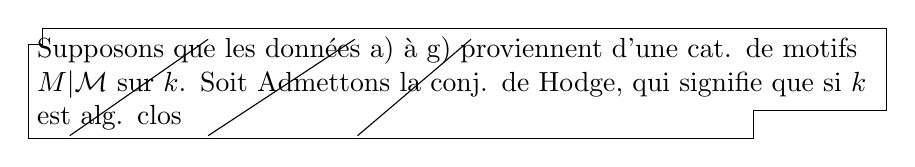
\begin{tikzpicture}[x=1cm,y=1cm]
\node[inner sep=3pt,text width=.88\linewidth,align=left] (oldblock) {\deleted{Supposons que les données a) à g) proviennent d'une cat. de motifs $\unsure{M|\mathcal M}$ sur $k$. \unsure{Soit} Admettons la conj. de Hodge, qui signifie que si $k$ est alg. clos}};
\draw ([xshift=5pt]oldblock.north west) -- (oldblock.north east) -- ([yshift=10pt]oldblock.south east) -- ([xshift=-48pt,yshift=10pt]oldblock.south east) -- ([xshift=-48pt]oldblock.south east) -- (oldblock.south west) -- ([yshift=-6pt]oldblock.north west) -- ([xshift=5pt,yshift=-6pt]oldblock.north west) -- cycle;
\draw ([xshift=15pt,yshift=1pt]oldblock.south west) -- ([xshift=65pt,yshift=-4pt]oldblock.north west);
\draw ([xshift=65pt,yshift=1pt]oldblock.south west) -- ([xshift=118pt,yshift=-4pt]oldblock.north west);
\draw ([xshift=119pt,yshift=1pt]oldblock.south west) -- ([xshift=160pt,yshift=-4pt]oldblock.north west);
\end{tikzpicture}}

Soit $V_{\mathbb Q},\ V_{\mathbb C}=\sum_{pq}V^{pq}$ une structure de Hodge, et soit $G$ son gpe de Mumford-Tate, donc $G_{\mathbb C}\subset\underline{\mathrm{Aut}}_{\mathbb C}(V)$. Soit $V_k\unsure{\subset|\subseteq}V_{\mathbb C}$ une restriction des scalaires de $\mathbb C$ à $k\subset\mathbb C$, \deleted{\unsure{une}} \uline{compatible} avec la filtration naturelle de $V_{\mathbb C}$. Supposons que $(V_{\mathbb Q},\,V_{\mathbb C}=\sum V^{pq},\,V_k\subset V_{\mathbb C})$ provienne d'un motif sur \uuline{$k$}. \inserted{\deleted{Admettant}} \deleted{et admettons la conj. \unsure{de H.|de h}} \deleted{Alors}

\unsure{Le} gpe de Galois motivique de ce dernier, \unsure{rel.} à $T_{\mathrm{DR}}$, est \unsure{une|un} \deleted{forme} \inserted{groupe} $G'$ \unsure{déf}/$k$, \deleted{de $G_{\mathbb C}$,} et en vertu de \uline{conj. de Hodge} on doit avoir $G'_{\mathbb C}\unsure{=|\subset|\supset}G^\circ_{\mathbb C}$. \deleted{(\unsure{d'après} \illegible{2})} \unsure{En} d'autres termes, il faut que $G^\circ_{\mathbb C}$ soit ``définissable sur $k$ via $V_k\subset V_{\mathbb C}$'' ; c'est une condition \unsure{très|très ;} \unsure{fort|; fort} non triviale ! Lorsque $k$ est \unsure{alg.|algéb.} clos, il faudra \deleted{\unsure{en}} $G'_{\mathbb C}=G_{\mathbb C}$, ce qu'on peut exprimer en disant que $\unsure{\forall|H}$ \deleted{\unsure{invariant}} élément d'un ${\unsure{\bigotimes|\otimes}}_{\mathbb Q}^{\unsure{n|m}}(V'\otimes_{\mathbb Q}V)$ invariant sous $G$ (i.e. de bidegré $0$) est \unsure{nécessairement|nécéssairement} dans $\bigotimes_{\unsure{k'|\bar k}}^{\unsure{n|m}}(V'_{\unsure{k'|\bar k}}\otimes_{\bar k}V_{\unsure{k'|K'}})$\unsure{!} ; si $k$ général, il faut \deleted{remplacer $k$ par une extension} \inserted{donc $\exists$ extension finie $k'$ de $k$,} ayant la \unsure{vertu|même} \unsure{précédente|propriété}. Ce sont encore des conditions très restrictives sur la structure envisagée. Elles ne sont certainement pas suffisantes (\unsure{faire|pour} $k=\mathbb Q$, $V_k=V_{\mathbb Q}$, ce n'est en général pas possible
\figure{\begin{tikzpicture}[x=1pt,y=1pt]
\draw[dash pattern=on 8pt off 4pt] (0,0) -- (49,0);
\draw (55,6) -- (60,6) -- (61,0) -- (55,0);
\end{tikzpicture}}
% paper watermark, sideways, second fragment clipped at the lower edge
{\centering \textsc{Strong}\\
\textit{\unsure{uy|ny|y} 1808}\par}
% archive sheet number: 30
\scanpage{32}
Il faut donc compléter les conditions \unsure{néc.|nèc.|nec.} \unsure{précédentes|précèdentes} par des \deleted{\unsure{conjectures}} \inserted{conditions} du type ``\unsure{conj.} de transcendance''\unsure{,.|,} pour éliminer le contre-exemple \unsure{précédent|précèdent}.

% paper watermark, sideways
{\centering \textsc{Extra Strong}\\
\textit{Ma\unsure{in|nn}\unsure{ol|on}\unsure{uy|ny|y} 1808}\par}
% archive sheet number: 31
\scanpage{34}
\margin{\begin{tabular}{|l@{}}Situation abstraite du\\double réseau\\\hline\end{tabular}}
$\unsure{\mathcal M|M}$ $\otimes$-catégorie sur corps $k$,
\diagram{\begin{tikzcd}[ampersand replacement=\&,row sep=1pt,column sep=5pt]
{} \& L\arrow[dd,no head] \& {}\\
K\arrow[ur,no head]\arrow[dr,no head]\arrow[r,no head,shorten >=3pt] \& {} \& \deleted{\unsure{\neq|?}}\\
{} \& k \& {}
\end{tikzcd}}
diagramme de corps

\[
\begin{aligned}
T&\quad\text{foncteur \unsure{fibre|fibré} }/k\\
T'&\quad\rule{2.8cm}{.35pt}\quad K\quad\text{\deleted{extension de $k$}}\\
\varphi&\colon T\otimes_k L\simeq T'\otimes_K L\qquad\otimes\ \text{isom.}
\end{aligned}
\]

Soit
\[
\left\{\begin{aligned}
G&=\underline{\mathrm{Aut}}_{\otimes}(T)&\quad&\text{gpe affine sur }k\\
P&=\underline{\mathrm{Isom}}_{\otimes}(T_K,T')&&\text{torseur à droite sous }G_K\\
\varphi&\in P(L)
\end{aligned}\right.
\]
Ces données permettent de réconstituer $\mathcal M,T,T',\varphi$.

Supposons d'abord $P$ trivial, et soit $\unsure{\xi|\zeta}\in P(K)\subset P(\deleted{\unsure{K|k}}L)$. On a donc $\xi=\varphi g,\quad g\in G(L)$. Si on remplace $\xi$ par $\xi'$, on aura $\xi'=\xi a$, $a\in G(K)$, donc $g$ remplacé par $ga$. Donc on définit canoniquement
\[
\dot g\in G(L)/G(K),
\]
et on voit que la connaissance de $(G,\dot g)$ équivaut à celle de $(G,P,\varphi)$. Soit alors $V$ un $G$-module, alors le réseau $T'(V)\subset V\otimes_k L$ n'est autre que $g(V\otimes_k K)$. On a
\[
V\cap T'(V)=\{\,x\in V\unsure{\}|\imath}\mid g^{-1}x\in V\otimes_k K\,\}.
\]
\deleted{Soit $y=g^{-1}x$}

\unsure{S} \deleted{Donc Si \unsure{on} $k$ est un} Soit $\unsure{\gamma|y}$ l'image de $g$ dans $G_K$ (\unsure{connue mod|soumise aux} \unsure{translations} à droite par $a\in G(K)$), $\underset{\substack{\text{\unsure{l'adh.|adh.}}\\\text{\unsure{de|dans}}\ T_K}}{\overline{\{\gamma\}}}=T_K\subset G_K$, \inserted{Soit $y=g^{-1}x$ ;} alors \deleted{\unsure{pour tt}} comme \deleted{$\unsure{\gamma\,\mathrm{Tra}}$} $\gamma\in\mathrm{Transp}_{G_K}(x,y)(L)$, on a $T_K\subset\mathrm{Transp}_{G_K}(x,y)$, \deleted{\unsure{pt} $s$ de $T_K$ à valeurs ds une alg. sur $K$, \illegible{1}} donc pour deux \deleted{\unsure{tel}} \deleted{$s^{-1}x=\unsure{g|t}y$ donc si} $s,t$ \deleted{sont deux tels points on a} de $T_K$ (à val. dans une $K$-alg. \unsure{quelc.}) on a $s^{-1}\unsure{a|x}=t^{-1}x$ i.e. $ts^{-1}x=a$ i.e. $ts^{-1}\in(G_K)_x=(G_x)_K$.

Soit donc $R$ \unsure{:} l'adhérence de l'image de $T_K\times T_K\underset{\deleted{\unsure{g|u}}}{\longrightarrow}G_K$ par $(s,t)\unsure{\mathrel{-}|\longrightarrow}ts^{-1}$ ; il est immédiat qu'elle ne dépend pas du choix de $g$ mod $G(K)$, \deleted{et que}
\[
\boxed{R\subset G_K}
\]
% paper watermark, sideways, reversed on this face
{\centering \textsc{\unsure{Extra} Strong}\\
\textit{Ma\unsure{in|nn}\unsure{ol|on}\unsure{uy|ny|y} 1808}\par}
% archive sheet number: 33
\scanpage{35}
l'on doit avoir, si $\unsure{x|a}\in V\cap T'(\unsure{V|W})$, $R_K\subset G_{x\,K}$. L'inverse est vrai, car comme $T_K$ est fid. plat \unsure{par|sur} $K$, on voit par descente que les \unsure{pts} (\unsure{à coeff. ds des|à coeff. dans des} $K$-alg. quelconques $\Lambda$) $s.x$ $(s\in T_K(\Lambda))$ proviennent d'un pt bien déterminé de $V_K$. Or soit \deleted{\unsure{$\xi$}}
\[
S_{\unsure{K|k}}=\overline{\unsure{\varphi|p}(R_K)}\qquad p\colon G_K\unsure{\mathrel{-}|\longrightarrow}G,
\]
et soit $H$ le ss-gpe algébrique \inserted{fermé} de $G$ engendré par $S$. On a donc
\[
x\in V\cap T'(V)\quad\Longleftrightarrow\quad x\in V_{\deleted{\unsure{x|0}}}^{H}\quad \deleted{\unsure{H|\forall}\unsure{\subset|\in}\unsure{G}\ \unsure{H_x|H}\ \text{\unsure{tous|tels}}}.
\]

Par suite, pour que \deleted{les invariants} pour tout $V$, on ait $V\cap T'(V)=V^G$, i.e. que le foncteur $\mathrm{Rep}(G)=\unsure{\mathcal M|M}\longrightarrow$ (structures vectorielles mixtes pour $L/K/k)$ soit pl. fid, il \unsure{n. f. et s.|f. et s.} que pour $\unsure{\forall|H}\,V$, \deleted{les invariants} on ait
\[
V^H=V^G.
\]

Supposons $P$ quelconque. On a l'\unsure{hom|hom.} canonique de bitorseurs
\[
\deleted{\unsure{\underline{\mathrm{Isom}}|{\mathrm{Isom}}}_{\unsure{\otimes}}(\unsure{T'|T},T_K))}
\]
\diagram{\begin{tikzcd}[ampersand replacement=\&,row sep=small]
P\mathbin{\unsure{\times|\otimes}}_K P\arrow[r] \& G_K\\
(v,u)\arrow[r,mapsto] \& v^{-1}u
\end{tikzcd}}
\deleted{\unsure{induisant}}
\[
\deleted{P_L^{\unsure{a|G}}\times P_L\mathrel{\unsure{-|\longrightarrow}}G_L}
\]
donc $\varphi\colon\mathrm{Spec}\,L\longrightarrow P$ (un $\mathrm{Spec}\,K$-\unsure{mor.|m.}, bien sûr) s'en déduit \deleted{de, grâce à l'isom $P_L\simeq G_L$}
\[
\mathrm{Spec}(L)\times_{\mathrm{Spec}\,K}\mathrm{Spec}(L)\mathrel{\unsure{-|\longrightarrow}}
P\times_{\mathrm{Spec}\,\unsure{K|k}}P\longrightarrow G_K\,;
\]
l'image fermée $\deleted{\unsure{P|R}}R_K$ est donc définie intrinsèquement. On vérifie encore (par descente \unsure{platisation|fidèlement|plate}) que \deleted{\unsure{p}} l'on a, pour tt $G$-module $V$
\[
\deleted{\unsure{x\in}}V\cap T'(V)=\{\,x\in V,\mid R_K\subset G_{x\,K}\,\}.
\]
Définissant $H$ comme ci-dessus, on trouve donc
\[
V\cap T'(V)=V^H,
\]
et la \unsure{$\overline{\mathrm m}$|même} conclusion que plus haut ....
% paper watermark, sideways
{\centering \textsc{Extra Strong}\\
\textit{Ma\unsure{in|nn}\unsure{ol|on}\unsure{uy|ny|y} 1808}\par}
% archive sheet number: 34
\scanpage{37}
% archive sheet number: 36
$K\subset\mathbb C$, $\bar K$ clôture alg. dans $\mathbb C$, $\unsure{\pi_1|\Pi_1}=\pi_1(\mathrm{Spec}\,K,\bar K)=\mathrm{Gal}(\bar K/K)$, $\unsure{A|\mathcal A}={}$anneau des adèles ``finis'' de $\mathbb Q$. On \unsure{$^{1}$|$^{l}$}considère une catégorie de motifs sur $K$, de type fini, et le groupe de Galois \inserted{$G$} associé au foncteur de Betti. Cela donne naissance aux structures suivantes.

% Diagram across the head of the sheet; the small boxes share their frames' corners.
\diagram{\resizebox{\linewidth}{!}{\begin{tikzcd}[ampersand replacement=\&,column sep=4pt,row sep=7pt,execute at end picture={
 \draw ([xshift=-5pt,yshift=6pt]gd.north west) rectangle ([xshift=5pt,yshift=-8pt]gp.east |- gm.south);
 \node[draw,anchor=south east,inner sep=1pt] at ([xshift=5pt,yshift=-8pt]gp.east |- gm.south) {$D$};
 \draw ([xshift=-5pt,yshift=6pt]p.north west) rectangle ([xshift=5pt,yshift=-12pt]g.south east);
 \node[draw,anchor=south east,inner sep=1pt] at ([xshift=5pt,yshift=-12pt]g.south east) {$B$};
 \draw (p.south) -- (avec.north);
 \draw (conn.center) ellipse [x radius=38pt,y radius=13pt];
 \draw (pc.south) -- (ptc.north);
 \draw (qc.south) -- (ptq.north);
 \draw (ptc.center) ellipse [x radius=37pt,y radius=14pt];
 \node[draw,anchor=south east,inner sep=1pt] at ([xshift=5pt,yshift=-3pt]ptc.south east) {$C$};
 \node[draw,anchor=south east,inner sep=1pt] at (ga.south east) {$A$};
}]
 |[alias=gd]| G''_K \arrow[r,phantom,"{\unsure{\supset|\to}}" description] \& H''_K\arrow[r,dash,dashed] \& Q\arrow[r,dash,dashed] \& H'_K \&[-4pt] {\subset} \&[-4pt] |[alias=gp]| G'_K\arrow[r,dash,dashed] \& |[alias=p]| P\arrow[r,dash,dashed] \& |[alias=g]| G_K \&[13pt] |[alias=pc]| P_{\mathbb C} \& G_{\mathbb C} \& |[alias=qc]| Q_{\mathbb C} \&[8pt] |[draw,alias=ga,minimum width=34pt,minimum height=24pt]| G\\
 |[alias=gm]| \mathbb G_m\arrow[u,shift left=1,"i_1"]\arrow[u,shift right=1,"i_2"'] \& \& \& \& \& \& |[alias=avec]| \text{avec} \& \& |[alias=ptc]| \begin{gathered}\text{avec pt }\deleted{\unsure{\xi|a}}\ \alpha\\\text{rat}/\mathbb C,\ \text{de}\end{gathered} \& \& |[alias=ptq]| \begin{gathered}\text{avec pt }\unsure{\xi_1|\alpha_1}\\\text{rat}/\mathbb C,\end{gathered} \& \\
 \& \& \& \& \& \& |[alias=conn]| \begin{gathered}\text{connexion absolue}\\\text{intégrable}\end{gathered} \& \& \text{sorte que} \& \& \& \\
 \& \& \& \& \& \& \begin{gathered}\text{invariante}\\\text{par }G_K\\{}[\,\text{NB structure vide}\\\text{si }K\ \text{abst. alg}\,]\end{gathered} \& \& \& \& \&
\end{tikzcd}}}

\diagram{\begin{tikzcd}[ampersand replacement=\&,column sep=25pt,execute at end picture={\draw ([xshift=-3pt,yshift=6pt]pu.north west) rectangle ([xshift=4pt,yshift=-4pt]gu.south east); \node[draw,anchor=south east,inner sep=1pt] at ([xshift=4pt,yshift=-4pt]gu.south east) {$\unsure{F|E|G}$};}]
 |[alias=pu]| \pi_1 \arrow[r,"{\substack{\deleted{\unsure{v|w}}\\u}}"] \& |[alias=gu]| G(A)
\end{tikzcd}}
\[
 \deleted{(\pi_1)_{\mathbb Q}\xrightarrow{\unsure{v|u}}G/G^\circ\quad\text{i.e.}\quad\pi_1\to(G/G^\circ)(\mathbb Q)}
\]

\uline{NB} La donnée \deleted{\unsure{principale}} compliquée $\boxed D$ peut être remplacée par la ``donnée subordonnée'' $\boxed E$, \uline{soumise} à la condition d'être ``compatible'' avec $A,B,C$

a) la connexion absolue définit
\[
 \omega\in\Omega^1_{\mathbb C/\mathbb Q}\otimes_{\mathbb Q}{\unsure{\mathfrak g|g}}_{\mathbb Q}
\]

b)
\diagram{\begin{tikzcd}[ampersand replacement=\&,column sep=0pt,row sep=0pt]
 G'_{\unsure{1|{}}} \& \otimes_K\mathbb C \&[5pt] \simeq \&[5pt] G_{\mathbb C}\\
 {\rotatebox{90}{$\subset$}} \& \& \&\\
 H' \& \otimes_K\mathbb C \& \&\\
 {\rotatebox{90}{$\simeq$}} \& \& \&\\
 H'' \& \otimes_K\mathbb C \& \&\\
 {\rotatebox{90}{$\simeq$}} \& \& \&\\
 G''_{\unsure{1|{}}} \& \otimes_K\mathbb C \& \simeq \& G_{\mathbb C}
\end{tikzcd}}

c) d'où des hom
\diagram{\begin{tikzcd}[ampersand replacement=\&,row sep=1pt,column sep=8pt]
 \& \& \boxed E\arrow[d]\\
 i_1^{\mathbb C},i_2^{\mathbb C}:\mathbb G_{m\,\mathbb C}\arrow[r] \& G_{\mathbb C} \& {}
\end{tikzcd}}

d) On a, pour un modèle régulier convenable $S$ de $K$, de type fini sur $\mathbb Z$ (supposons $K$ de t.f. sur $\mathbb Q$)
\diagram{\begin{tikzcd}[ampersand replacement=\&,column sep=16pt,row sep=5pt,execute at end picture={\draw ([xshift=-4pt]ds.south east) |- ([xshift=2pt,yshift=2pt]geom.north);}]
 \& \& \boxed G\\
 |[alias=ds]| \pi_1(S(\mathbb C),{\unsure{\xi|\zeta}})\arrow[r,"w"] \& G(\mathbb C). \&\\
 |[alias=geom]| \begin{gathered}\text{pt géom}\\\text{déduit de}\\\text{l'inclusion}\\K\subset\mathbb C\end{gathered} \& \begin{gathered}{}[\,\text{NB : structure}\\\text{vide si }K\text{ est}\\\text{abst. alg.}\,]\end{gathered}\&
\end{tikzcd}}

% The line running from e) meets the lower right corner of the boxed consequence.
\diagram{\resizebox{\linewidth}{!}{\begin{tikzcd}[ampersand replacement=\&,column sep=9pt,row sep=5pt,execute at end picture={
 \coordinate (cl) at ([xshift=-4pt]lh.west);
 \coordinate (cr) at ([xshift=6pt]qr.east);
 \draw ([yshift=3pt]cl |- lh.north) rectangle ([yshift=-4pt]cr |- lb.south);
 \draw ([xshift=-13pt,yshift=-9pt]lh.west) circle [radius=2pt];
 \draw ([xshift=-13pt,yshift=-9pt]lh.west) -- ([xshift=1pt,yshift=5pt]lh.north west);
 \draw[rounded corners=6pt] ([xshift=-8pt,yshift=1pt]eb.south west) -- ([xshift=-4pt,yshift=-4pt]cr |- lb.south) -- ([xshift=-6pt,yshift=6pt]et.north west) -- ([xshift=8pt,yshift=4pt]et.north east) -- ([xshift=10pt,yshift=-1pt]eb.south east) -- ([xshift=-8pt,yshift=-2pt]eb.south west) -- cycle;
}]
 |[alias=lh]| \text{Il en résulte aussi que le diagramme} \& {} \&[25pt] {}\\
 \pi_1(S(\mathbb C),\xi)\arrow[r]\arrow[d,"\mathrm{can.}"] \& |[alias=qr]| G(\mathbb Q)\arrow[d] \& |[alias=et]| \begin{gathered}\text{e) }P/G^\circ\text{ est un}\\\text{torseur sur }K,\ \text{de}\end{gathered}\\
 \pi_1(S,\xi)\arrow[r,"v"] \& G/G^\circ(\mathbb Q) \& \begin{gathered}\text{groupe }G/G^\circ,\ \text{ponctué}\\\text{par }\xi:K\to\mathbb C,\ \text{donc}\end{gathered}\\
 |[alias=lb]| \text{est commutatif} \& {} \& |[alias=eb]| \begin{gathered}\text{définit}\quad v:\pi_1\longrightarrow(G/G^\circ)(\mathbb Q)\\\text{i.e.}\quad\pi_1\longrightarrow(G/G^\circ)_{\mathbb Q}\end{gathered}
\end{tikzcd}}}

\uline{Propriétés}

1) $i_2^{\mathbb C}=\overline{i_1^{\mathbb C}}$ (donc $\unsure{\alpha_1|\alpha}$ est connu quand on connaît $\alpha$)

2) $\pi_1(S(\mathbb C),\xi)\to G(\mathbb C)$ se factorise par $G(\mathbb Q)$, \deleted{et on a \unsure{compatibilité}}

3) $\pi_1\to G(A)$ se factorise par $\pi_1(S,\xi)\unsure{\mathrel{-}|\to}G(A)$ pour $S$ convenable

4) les diagr.
\diagram{\begin{tikzcd}[ampersand replacement=\&,column sep=27pt]
 \pi_1(\deleted{\unsure{S|C}}S(\mathbb C)\deleted{\unsure{,\xi|)}} ,\xi)\arrow[r,"{\deleted{\unsure{\pi_1|u}}}","w"']\arrow[d,"\mathrm{can.}"] \& G(\mathbb Q)\arrow[d,"\mathrm{can.}"]\\
 \pi_1(S,\xi)\arrow[r,"u"] \& G(A)
\end{tikzcd}\hspace{5pt}\begin{tikzcd}[ampersand replacement=\&,column sep=13pt]
 \pi_1\arrow[r,"v"]\arrow[d,"u"] \& G/\deleted{\unsure{G'|G}}G^\circ(\mathbb Q)\arrow[d]\\
 \deleted{\unsure{u|G}}G(A)\arrow[r] \& (G/G^\circ)(A)
\end{tikzcd}}
\unsure{sont|\deleted{sont}} commutatifs. \unsure{!|/}

5) Le composé $\pi_1(S,\xi)\unsure{\mathrel{-}|\to}G(A)\xrightarrow{\unsure{\varepsilon|\epsilon}}A^*$ est l'hom défini par l'action de $\pi_1(S,\xi)$ sur les racines de l'unité.

% This addition occupies the lower right of the sheet. Its linking stroke begins after 5).
\figure{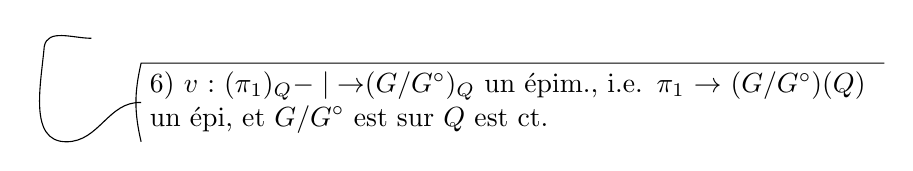
\begin{tikzpicture}
 \node[inner sep=3pt,text width=.76\linewidth,align=left] (addsix)
 {\inserted{6) $v:(\pi_1)_{\mathbb Q}\unsure{\mathrel{-}|\to}(G/G^\circ)_{\mathbb Q}$ un épim., i.e. $\pi_1\to(G/G^\circ)(\mathbb Q)$ un épi, et $G/G^\circ$ \deleted{\unsure{est}} sur $\mathbb Q$ est \uuline{ct}.}};
 \draw (addsix.north east) -- (addsix.north west) to[bend right=13] (addsix.south west);
 \draw (addsix.west) to[out=178,in=0] ([xshift=-27pt]addsix.south west) to[out=180,in=-95] ([xshift=-35pt,yshift=6pt]addsix.north west) to[out=80,in=180] ([xshift=-18pt,yshift=9pt]addsix.north west);
\end{tikzpicture}}

\deleted{\unsure{6|7}}7) Pour tout point fermé $s$ de $S$, l'élément de \unsure{frobénius|frobènius} $f_s$ de $\pi_1(S,\xi)$ a \deleted{comme image} \inserted{une} classe dans $G(A)$ \inserted{qui correspond à} l'image d'une classe de conjugaison de $G\deleted{\unsure{(A)|_{\mathbb Q}}}$ (redonne Weil \unsure{...|....}).

% slanted
\margin{devra être \unsure{précisé|precisé} ...}

\deleted{\unsure{7|8}}8) $G_{\mathbb R}$ muni de $i_1^{\mathbb C},i_2^{\mathbb C}$ de c) est un \uline{groupe de Hodge}.

\deleted{\unsure{8|9}}9) (\unsure{Modulo Tate|Modules Tate}) Pour tout $\unsure{l|\ell}$, l'image de $\pi_1\unsure{\xi|K|\mathopen{(}}$ dans $G(\mathbb Q_l)$ est un sous-groupe opérant de façon $\unsure{\frac12|\text{semi}}$ simple sur tout \deleted{\unsure{produit|foncteur|générateur}} $V\otimes_{\mathbb Q}\mathbb Q_l$ \deleted{\unsure{engendre|engendré} $\mathbb Q_l$ \unsure{comme}}, (ou un tel, avec $\deleted{\unsure{V|D}}V$ \deleted{\unsure{semi|seul}} fidèle), et son enveloppe algébrique est $G_{\mathbb Q_l}$.

\deleted{\unsure{Le composé} $\pi_1\to G(A)\to G(\mathbb Q)\unsure{\mathrel{-}|\to}G/G^\circ$}

% paper watermark, sideways
{\centering \textsc{Extra \unsure{Strong}}\\
\textit{Ma\unsure{in|nn}\unsure{ol|on}\unsure{uy|ny|y} 1808}\par}
